Il processo di fissione nucleare è un processo legato alla stabilità di nuclei. Processo che produce energia. Partendo dal grafico di energia di legame per nucleone.
%IMMAGINE el
\begin{figure}[htp!]
  \centering
  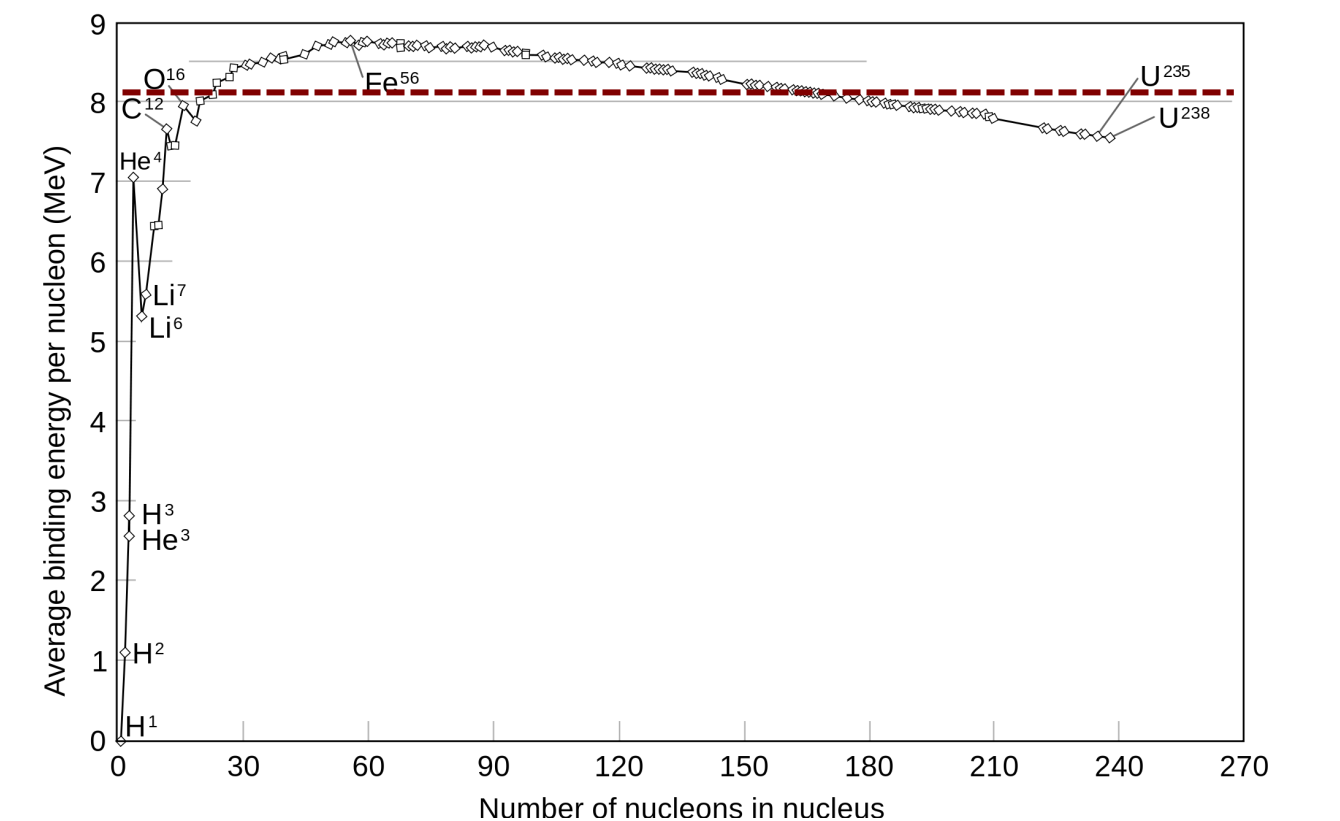
\includegraphics[scale=0.4]{Lezione2/el.png} 
\end{figure}
In questo caso stiamo studiando la parte alta del grafico e cioè nella zona a grande $A$ della curva di energia di legame. Alla fine di questa curva notiamo che abbiamo nulcei che hanno un'energia di legame più bassa rispetto a quella dei precedenti. Quindi per questi nuclei potrebbe essere più conveniente dividersi e formare due nuclei più leggeri. In quanto l'energia di legame per nucleone è più alta in modulo ma l'energia di legame $B.E.$ è più bassa con il segno e quindi energeticamente favorita. I nuclei pesanti possono scindersi in nuclei più leggeri e più legati liberando energia. Questo processo è possibile per $A\ge120$ circa. Questo processo non avviene spontaneamente a causa della solita barriera di potenziale. Questo è dovuto alla stabilità dei nuclei rispetto alla repulsione elettrostatica. Questo rientra anche nella formula di Bethe-Weizs\"acker questa discesa di energia di legame per nucleone è proprio dovuta alla repulsione elettrostatica. Qui gioca un doppio ruolo. Mi permette la fissione nucleare ma sarà anche quella che poi non permette che questo processo sia spontaneo.

Per superare questa barriera elettrostatica è necessario eccitare il nucleo attraverso l'interazione con neutroni.
\subsection{Fissione nucleare}
La fissione è il proceso in cui un nucleo si spezza in frammenti più piccoli. Il caso più semplice:
\begin{equation*}
    \ch{^A_ZX} \rightarrow \ch{^{A_1}_{Z_1}X} + \ch{^{A_2}_{Z_2}X} + Q_{fiss}
\end{equation*}
Ovviamente abbiamo il vincolo che:
\begin{equation*}
    A=A_1+A_2 \qquad \quad Z=Z_1+Z_2
\end{equation*}
Il numero di massa totale e la carica deve conservarsi. L'energia del processo di fissione si trova attraverso la differenza di massa
\begin{equation*}
    Q_{fiss}=M(A,Z)-M(A_1,Z_1)-M(A_2,Z_2)
\end{equation*}
Purchè la fissione sia permessa, dal punto di vista energetico deve essere $Q_{fiss}>0$ perchè questa quantità rappresenta l'energia cinetica che io ho a disposizione dei miei frammenti. Utilizzando l'energia di legame:
\begin{equation*}
    Q_{fiss}=B(A,Z)-B(A_1,Z_1)-B(A_2,Z_2)
\end{equation*}
Dove l'energia di legame è data dalla formula di Bethe-Weizs\"acker
\begin{equation*}
    B(A,Z)=-a_1A+a_2A^{\frac{2}{3}}+a_3\frac{Z^2}{A^{\frac{1}{3}}}+a_4\frac{(A-2Z)^2}{A}\pm a_5A^{-\frac{3}{4}}
\end{equation*}
Abbiamo visto che contiene il termine che dipende dalla superficie che tenderebbe a favorire nuclei grandi però c'è il termine di repulsione coulombiana che tende a sopprimere nuclei troppo grandi. Perchè cresce come una $Z^2$  a differenza del termine di legame nucleare che cresce linearmente.

L'energia disponibile è approssimativamente $0.9\,MeV$ per nucleo. Questo perchè noi partiamo da un numero $Z$ di circa $240$ quindi a grosso modo ci aspettiamo che i frammenti di decadimento siano in una zona attorno a $Z=120$ (circa la metà della massa iniziale) la differenza di energia di legame per nucleone è circa $0.9\,MeV$. Quindi se utilizzo magari l'Uranio-240 ottengo qualcosa come circa $200\,MeV$ di energia per fissione. La densità di energia immagazzinata è molto maggiore di quella di combustibili chimichi $20-50\,MJ/kg$. Invece, ad esempio $1\,g$ di materia ha circa $N_A$ nucleoni, quindi $1\,kg$ di materiale ha circa $6\times10^{26}$ nucleoni. La densità di energia, moltilicando l'energia per nucleone per il numero di nucleoni: $5.4\times10^{26}\, MeV/kg$. Ora trasformo l'unità di misura da $MeV$ a $J$: $1\,MeV=(10^6e)\,J=1.6\times10^{-13}J$ a questo punto moltiplico questo fattore di conversione ottengo che la densità di energia è: $8.6\times10^{13} \,J/kg$. Ovvero $8.6\times10^7\,MJ/kg$. Quindi ho 6 ordini di grandezza maggiore rispetto a quella di combustibile fossile. Un milione di volte maggiore!
%IMMAGINE mem
\begin{figure}[htp!]
  \centering
  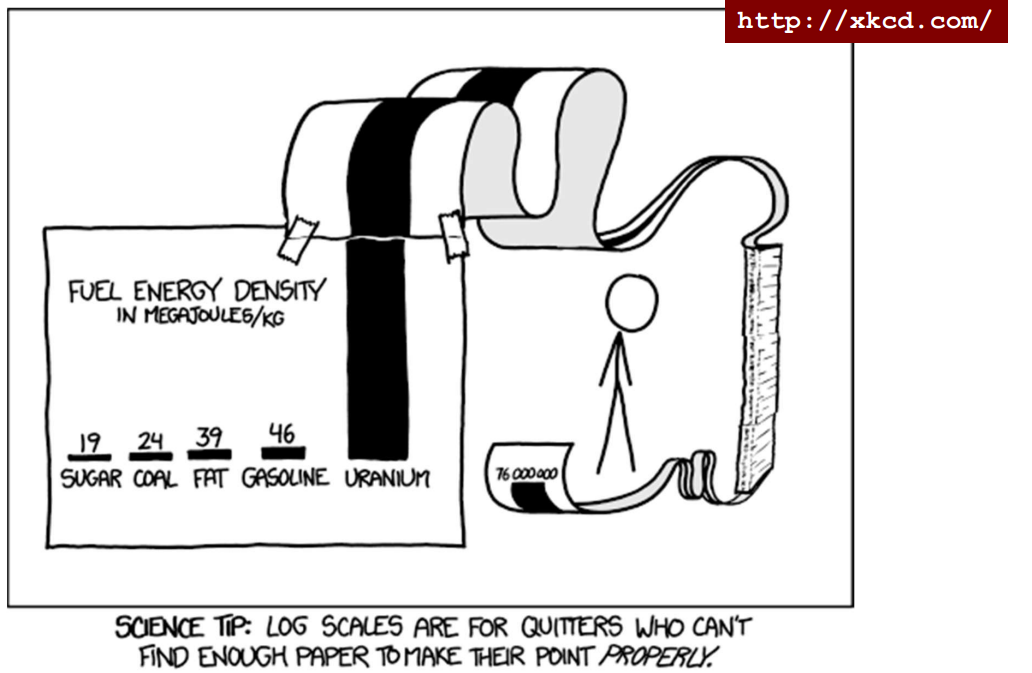
\includegraphics[scale=0.3]{Lezione5/mem.png} 
\end{figure}
\subsection{Processo di fissione}
Possiamo visualizzare il processo di fissione come la separazione di una goccia di liquido nucleare:
%IMMAGINE gocc
\begin{figure}[htp!]
  \centering
  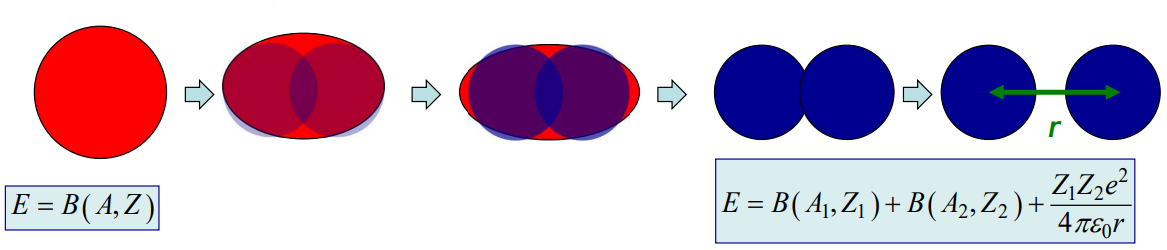
\includegraphics[scale=0.5]{Lezione5/gocc.png} 
\end{figure}
e quindi possiamo pensarla come una goccia di liquido che si separa in due. Quindi parto da un nucleo unico che ha una certa massa (un certo $Z$) questo nucleo inizia a deformarsi e a crearsi due zone differenti e alla fine si separano e in più si allontanano visto che sono carichi allo stesso modo respingendosi e allontanandosi. Finita la separazione avrò che la forza Coulombiana tenderà a seprararli facendo acquistare energia cinetica. L'energia del sistema quindi si evolve da quella dovuta all'energia di legame del nucleo originale a quella dei due nuclei separati.
%IMMAGINE pot
\begin{figure}[htp!]
  \centering
  
\includegraphics[scale=0.6]{Lezione5/pot.png} 
\end{figure}
Dal grafico del potenziale si vede l'andamento come $\frac{1}{r}$ dopo che i due nuclei si sono separati. La mia energia potenziale presenta una barriera o decresce esponenzialmente? Nel primo caso posso capire che il processo potrebbe avvenire facilmente se non spontaneamente mentre per quanto riguarda il secondo caso se devo superare una barriera di potenziale. La risposta è ovvia. Se il nucleo esiste significa che deve essere in una situazione di equilibrio e quindi siamo nel secondo caso. Infatti il nucleo può esistere solo se lo stato iniziale è metastabile (in uno stato in cui almeno classicamente ci starebbe), in tal caso la fissione necessita di superare una barriera di potenziale.

Vado a vedere come questo modello a goccia si separa va a modificare la formula di Bethe-Weizs\"acker. I termini influenzati da una deformazione del nucleo sono: l'energia superficiale e l'energia di Coulomb. Quindi i termini moltiplicati ad $a_2$ e $a_3$. Gli altri termini rimangono invariati.
\subsubsection{Termine di superficie}
Quindi mi cambia la superficie, mi cambia l'energia coulombiana perchè dal momento che si allunga, mi cambia la distribuzione di carica e quindi mi cambia l'energia immagazzinata dal punto di vista coulombiano.
Assumiamo che un nucleo sferico di raggio R assuma una forma di ellissoide prolato. Introduciamo il parametro $\varepsilon$ che definisce una deformazione che mantiene costante il volume:
\begin{equation*}
    a=R(1+\varepsilon) \quad \Rightarrow \quad b=\frac{R}{\sqrt{1+\varepsilon}}
\end{equation*}
aumentando il parametro $a$ di una quantità $\varepsilon$ per mantenere il volume costante avrò anche $b$. Di conseguenza la superficie aumenta:
\begin{equation*}
    S=4\pi R^2\left(1+\frac{2}{5}\varepsilon^2\right)
\end{equation*}
Quindi nella formula di Bethe-Weizsacker il termine legato alla superficie diventa:
\begin{equation*}
    a_2A^{\frac{2}{3}} \rightarrow a_2A^{\frac{2}{3}}\left(1+\frac{2}{5}\varepsilon^2\right)
\end{equation*}Conlcudiamo che l'energia superficiale aumenta.
\subsubsection{Termine Coulombiano}
Per quando riguarda il termine dell'energia di legame dovuto alla repulsione elettrostatica, per una distribuzione sferica l'energia si calcola facilmente:
\begin{equation*}
    U=\frac{3}{5}\frac{1}{4\pi\varepsilon_0}\frac{Z^2e^2}{R}
\end{equation*}
il caso dell'ellisoide prolato è più complesso ma si ottiene:
\begin{equation*}
    U=\frac{3}{5}\frac{1}{4\pi\varepsilon_0}\frac{Z^2e^2}{R}\left(1-\frac{\varepsilon^2}{5}\right)
\end{equation*}
Assomiglia molto al potenziale della sfera con un termine correttivo negativo, questo è ovvio perchè sto andando ad allontanare parte delle cariche. Pertanto, per tenere conto della deformazione, nella formula di Bethe-Weizs\"acker si opera la sostituzione:
\begin{equation*}
    a_3\frac{Z^2}{A^{\frac{1}{3}}}\rightarrow a_3\frac{Z^2}{A^{\frac{1}{3}}}\left(1-\frac{\varepsilon^2}{5}\right)
\end{equation*}
Che rappresenta l'effetto della deformazione: l'energia elettrostatica diminuisce.
\subsubsection{Stabilità}
Quindi abbiamo due termini in competizione: l'energia superficiale che aumenta e l'energia elettrostatica che diminuisce. Dobbiamo vedere quale dei due vince. Vado a fare la differenza rispetto al nucleo sferico e ottengo che i termini in comune si cancellano:
\begin{equation*}
    \Delta E=\frac{2}{5}a_2A^{\frac{2}{3}}\left(1-\frac{a_3}{2a_2}\frac{Z^2}{A}\right)\varepsilon^2
\end{equation*}
ed è il segno di questo fattore che mi dice se modificando il nucleo l'energia di legame aumenta o diminuisce. Introducendo i valori delle costanti:
\begin{equation*}
    \Delta E\approx\frac{2}{5}a_2A^{\frac{2}{3}}\left(1-\frac{1}{50}\frac{Z^2}{A}\right)\varepsilon^2
\end{equation*}
Il nucleo sferico è stabile se $\Delta E > 0$ ovverso se la mia energia di legame sta aumentando, quindi è meno negativa e si sta avvicinando allo zero. La condizione di stabilità è pertanto:
\begin{equation*}
\frac{Z^2}{A}<50
\end{equation*}
Questa condizione è verificata anche per nuclei molto pesanti. Se avessi un nucleo con questo rapporto maggiore di 50 questo nucleo non si formerebbe perchè la repulsione coulombiana mi porterebbe a spezzare la mia goccia di liquido il prima possibile (vedi immagine del potenziale). Il nucleo sferico è uno stato stabile e questo porta al fatto che la fissione è un processo raro. Il fatto che il $\Delta E>0$ implica che sono in una condizione di minimo del potenziale e che quindi sono in una situazione di equilibrio stabile (vedi grafico).
\subsection{Vite medie parziali per fissione}
%IMMAGINE ggg ttr
\begin{figure}[htp!]
  \centering
  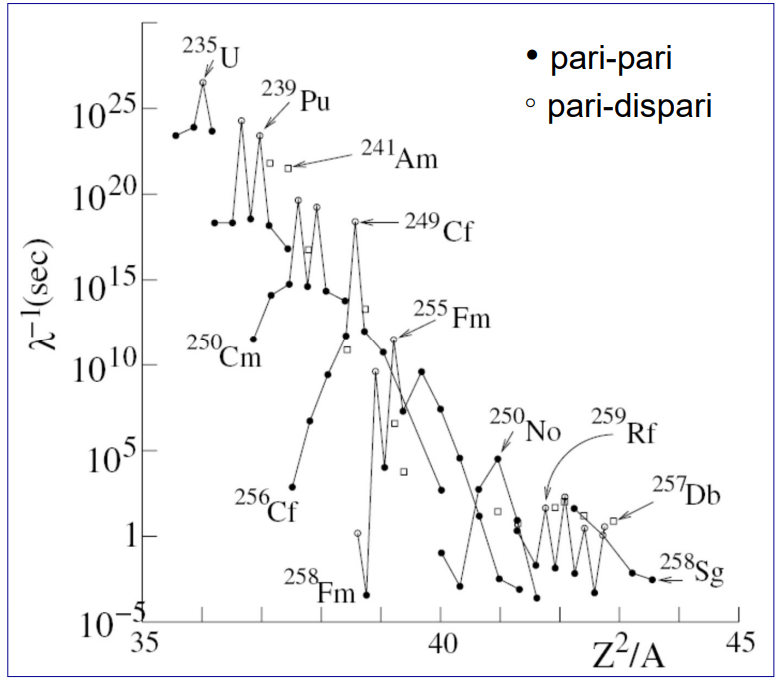
\includegraphics[scale=0.5]{Lezione5/ggg.png}
  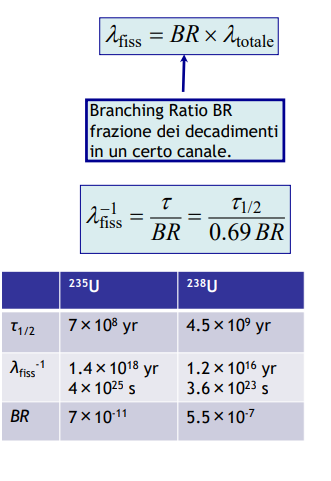
\includegraphics[scale=0.7]{Lezione5/ttr.png} 
\end{figure}
Sulle ascisse ho l'inverso della probabilità di decadimento. Che ci da un'idea su quanto sia importante quel determinato processo rispetto ad altri decadimenti. Ad esempio se non ci fosse decadimento alfa l'Uranio-235 avrebbe una vita media di $10^{25}\,s$ che è maggiore dell'età dell'universo quindi è un processo estremamente raro. Dalla tabella si può vedere il BR. Ad esempio ci dice che per l'Uranio-235 un solo nucleo su $7\times10^{11}$ fissiona mentre gli altri decadono alfa. Quindi il fatto che la configurazione a goccia è altamente stabile mi fa a sopprimere questo evento rendendolo molto poco probabile! (BR molto piccoli).
\subsection{Energia nucleare}
Il processo di fissione è alla base della produzione di energia nucleare. La fissione spontanea non è in grado di produrre una potenza apprezzabile: è necessario ricorrere a fissione indotta da neutroni (proprità della fissione e diverso comportamente dei materiali). Entra in gioco la reazione a catena quindi al possibile automantenimento della produzione di energia e al controllo della reazione. In questo entrano in gioco il moderatore e i neutroni ritardati.
\subsection{Fissione indotta}
Un evento di fissione rilascia una notevole quantità di energia: ad esempio per l'Uranio-238 ci aspettiamo: $0.9\,MeV/\text{nucleoni} \,\times\, 238\,\text{nucleone}=214\,MeV $. La potenza è però limitata, infatti per $1\,g$ di Uranio-238:
\begin{equation*}
    P=Q_{fiss}\frac{N_A}{A}\lambda_{fiss}\approx 200\, Mev\frac{6\times10^{23}}{238}\frac{1}{1.6\times10^{23}s}\approx4\,MeV/s \approx6\times10^{-13}W
\end{equation*}
Una quantità irrisoria soprattutto se confrontata con un altro processo come il decadimento $\alpha$:
\begin{equation*}
    P=Q_{fiss}\frac{N_A}{A}\frac{0.69}{\tau_{1/2}}\approx50000\,MeV/s\approx8\times10^{-9}W
\end{equation*}
4 ordini di grandezza di differenza. Visto che il tasso è così basso la fissione può essere indotta da collisioni con neutroni che pongono il nucleo in uno stato eccitato: in questo modo si riduce l'altezza della barriera di potenziale da superare. 

Un esempio di reazione:
\begin{equation*}
    n+\ch{^{235}_{92}U}\rightarrow\ch{^{236}_{92}U^*}\rightarrow\ch{^{137}_{53}I}+\ch{^{96}_{39}Y} +3n
\end{equation*}
Un neutrone che colpisce un nucleo di Uranio-235 che ha $Z=92$ lo porta in uno stato eccitato che si separa di fatto in due frammenti, conservando il numero $Z$ totale del nucleo iniziale mentre il numero di massa $A$ è leggermente minore, c'è un eccesso di neutroni che vengono prodotti in questo decadimento. La fissione non produce solo i nuclei risultanti ma anche neutroni. Il $Q_{fiss}=183\,MeV$. Pensando alla valle di stabilità, dopo questo processo ci sono dei nuclei con un numero abbondante di neutroni rispetto a quelli che servono al nucleo per rimanere stabile. Quindi, arrivati a questo punto, seguiranno dei decadimenti $\beta$ per arrivare ad uno stato di equilibrio producendo altra energia:
\begin{equation*}
    \ch{^{137}_{53}I}\xrightarrow[]{Q=6.0\,MeV}\ch{^{137}_{54}Xe}\xrightarrow[]{Q=4.1\,MeV}\ch{^{137}_{55}Cs}\xrightarrow[]{Q=1.1\,MeV}\ch{^{137}_{56}Ba}
\end{equation*}
\begin{equation*}
    \ch{^{96}_{39}Y}\xrightarrow[]{Q=7.1\,MeV}\ch{^{96}_{40}Zr}
\end{equation*}
Ci sono un sacco di possibili modi in cui il nucleo iniziale può dividersi in due, si veda i grafici:
%IMMAGINE pot
\begin{figure}[htp!]
  \centering
  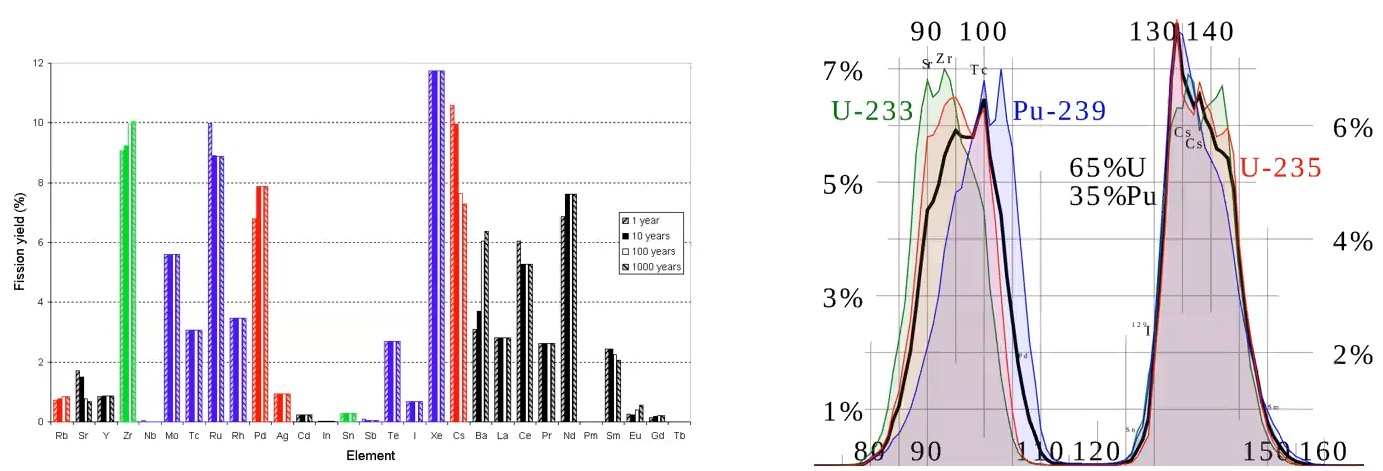
\includegraphics[scale=0.4]{Lezione5/figli.png} 
\end{figure}
i nuclei figli sono ricchi di neutroni quidi fatto decadimenti $\beta$ che rilasciano energia aggiuntiva, poi visto che il nucleo di partenza è ricco di neutroni vengono rilasciati altri neutroni. La ragione dell'assimetria dei due nuclei figli è facile da capire. Cosa rende difficile scindere il nucleo in due parti esattamente uguali? perchè se si va a vedere la barriera di potenziale. Se andiamo a vedere l'altezza della barriera di potenziale questa è il prodotto della carica dei nuclei figli, se andiamo a vedere come va il prodotto $Z_1$ e $Z_2$ con la condizione dello Z totale si va a scoprire che il caso in cui $Z_1=Z_2$ è un punto di massimo. Quindi è uno stato in cui ho la più alta barriera di potenziale. Mentre se ho le Z ben separate quello che succede è che la barriera di potenziale si abbassa. 

La fissione indotta dell'Uranio-235 è molto più probabile della fissione spontanea, succede che il nucleo $\ch{^{235}U}$ assorbe un neutrone molto lento (al limite fermo) e produce un nucelo di $\ch{^{236}U}$. Nel processo vengono rilasciati $6.3\,MeV$. Questa energia disponibile è sufficiente a produrre lo stato eccitato $\ch{^{236}U^*}$ (me ne servirebbero solo $5.7\, MeV$). Poichè il nucleo si trova in uno stato eccitato la barriera è più bassa e quindi, ricordiamo che la probabilità di effetto tunnel è una funzione esponenziale dell'altezza e della lunghezza della barriera. Di conseguenza ho una probabilità maggiore di superare la barriera.
Perchè abbiamo a disposizione tutta questa energia? L'Uranio-236 è un nucleo pari-pari mentre il nucleo precedente, l'Uranio-235 è un nucleo pari-dispari, quindi quando catturo un neutrone passo da dispari a pari-pari il risultato finale è che guadagno in $a_5$, in termini di profondità della mia energia di legame, quindi ho più energia disponibile per fare altre cose.
%IMMAGINE ggg ttr
\begin{figure}[htp!]
  \centering
  
\includegraphics[scale=0.65]{Lezione5/ds.png}
  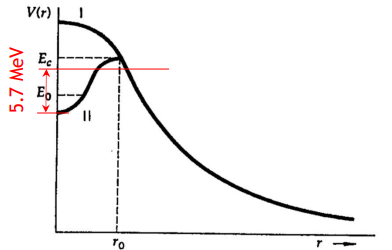
\includegraphics[scale=0.7]{Lezione5/ts.png} 
  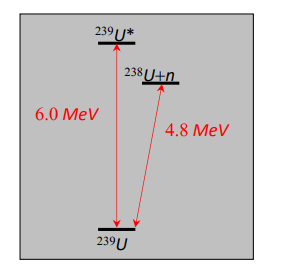
\includegraphics[scale=0.75]{Lezione5/uu.png} 
\end{figure}


Abbiamo utilizzato l'isotopo $\ch{^{235}U}$, che è molto meno abbondante dell'isotopo $\ch{^{238}U}$: i minerali di Uranio contengono solo una piccola percentuale di $\ch{^{235}U}$, circa solo il $0.7\%$. Per l'isotopo $\ch{^{238}U}$ l'equivalente processo di fissione indotta sarebbe quello rappresentato in figura, ma a differenza di prima l'energia liberata nella cattura non è sufficiente a produtte il primo stato eccitato $\ch{^{239}U^*}$. Il motivo di questa differenza si può comprendere ricordando l'ultimo termine dell'energia di legame della formula di Bethe-Weizs\"acker: nel primo caso abbiamo che il termine legato ad $a_5$ partiva da uno stato in cui era zero ad uno stato finale negativo per cui mi fa guadagnare energia di legame. Mentre per il secondo caso è negativo per il primo stato $\ch{^{238}U}$ (nucleo pari-pari) ma nullo nello stato finale. Quindi questa energia la perdo quando formo un nucleo dispari. Pertanto l'ultimo neutrone dell'isotopo $\ch{^{239}U}$ è "meno legato" e l'energia rilasciata nella cattura non è sufficiente per raggiungere il primo stato eccitato. Non c'è questo aumento di proabilità di fissione che abbiamo nell'Uranio-235. Nei reattori nucleari sentiamo parlare molto di più dell'Uranio-235 proprio per questo motivo, ed è un enorme peccato perchè è molta ridotta la quantità rispetto all'Uranio-238.

%IMMAGINE hh
\begin{figure}[htp!]
  \centering
  
\includegraphics[scale=0.7]{Lezione5/hh.png} 
\end{figure}

Dall'immagine si può visualizzare la sezione d'urto di due processi che sono in competizione. Uno per fissione e l'altro per cattura neutronica. Il primo sappiamo cosa è: viene catturato il neutrone e dopo la cattura il nucleo si divide. La seconda: il neutrone viene catturato quell'energia che viene liberata viene emessa tramite radiazione elettromagnetica, tramite produzione di raggi $\gamma$ (fotoni). Una volta che il nucleo cattura un neutrone può reagire o in un modo o nell'altro. Quale delle due è più probabile dipende dalla sezione d'urto. Bisogna stare attenti ad interpretare il grafico in quanto la sezione d'urto della cattura neutronica è stata abbassata di un fattore $100$ per evitare sovrapposizioni. Si nota che per alte energie il termine dominante è quello di fissione sia per l'Uranio-235 che per l'Uranio-238. Per l'isotopo $\ch{^{238}U}$ la soglia della fissione è molto elevata ($>2\,MeV$) questo perchè per creare lo stato eccitato e superare quindi la barriera di potenziale non mi basta l'energia di cattura del neutrone ma devo aggiungere qualcosa (in energia cinetica). Infatti si nota dal grafico come crolla la sezione d'urto della fissione per l'Uranio-238. Per l'Uranio-235 la fissione è possibile per ogni energia perchè l'energia di legame da sola è sufficiente per raggiungere lo stato eccitato. Quindi per neutroni lenti ($<1\,MeV$) la fissione è molto più frequente in $\ch{^{235}U}$ che dal grafico si vede che rimane alta d'appertutto.

Per l'Uranio-238 la competizione è presente solo ad alte energie, a basse energie abbiamo solo il processo di cattura neutronica in cui vengono "mangiati" i neutroni prodotti dalla fissione. Nel caso di Uranio-235 abbiamo sempre in competizione i due processi con uno che mi produce neutroni, l'altro che me li "mangia". La competizione di questi due termini e quello che mi determina l'andamento di fissione nucleare.
\subsection{Materiali fissili e materiali fertili}
L'Uranio-235 è l'unico materiale che conosciamo fissile, cioè è soggetto a fissione indotta con neutroni termici (neutroni a bassa energia). Esistono altri materiali ma sono molto meno presenti, ricordiamo che l'Uranio-235 è lo $0.7\%$ dell'uranio naturale. Ricordiamo che l'energia termica è espressa come: 
\begin{equation*}
    kT=25\,meV\quad T=300\,K
\end{equation*}
Però è possibile produrre altri materiali fissili dai "materiali fertili" ad esempio $\ch{^{239}Pu}$ e $\ch{^{233}U}$ da $\ch{^{238}U}$ e $\ch{^{232}Th}$, rispettivamente:
\begin{equation*}
    n+\ch{^{238}_{92}U}\,\to\,\ch{^{239}_{92}U}+\gamma \quad \Rightarrow\quad \ch{^{239}_{92}U}\,\to\, \ch{^{239}_{93}Np}+e^- \quad \Rightarrow\quad \ch{^{239}_{93}Np}\,\to\, \ch{^{239}_{94}Pu}+e^-
\end{equation*}
Dove dopo aver catturato il neutrone l'Uranio-238 si trasforma in Uranio-239 emettendo un fotone, successivamente avviene un decatimento $\beta$ con un tempo di dimezzamento: $\tau_{1/2}=23.4\,$minuti e dopo, con un tempo di dimezzamento $\tau_{1/2}=2.36\,$giorni trovo un altro materiale fissile, il Plutonio-239
\begin{equation*}
    n+\ch{^{232}_{90}Th}\,\to\,\ch{^{233}_{90}Th}+\gamma \quad \Rightarrow\quad \ch{^{233}_{90}Th}\,\to\, \ch{^{233}_{91}Pa}+e^- \quad \Rightarrow\quad \ch{^{233}_{91}Pa}\,\to\, \ch{^{233}_{92}U}+e^-
\end{equation*}
Lo stesso ragionamento vale per l'Uranio-233. Con tempi di dimezzamento $\tau_{1/2}=23.3\,$minuti per il primo e per il secondo $\tau_{1/2}=26.97\,$giorni.

Si nota che in entrambi i casi si passa da un nucleo pari pari che diventano dispari (quindi la cattura neutronica è predominante). Si nota anche che i primi decadimenti $\beta$ hanno un $Q_{val}$ più grande perchè siamo più lontani dalla valle di stabilità e quindi avvengono più rapidamenti. I decadimenti successivi invece impiegano più tempo.

Questo si può sfruttare ad esempio con un reattore che brucia $\ch{^{239}Pu}$ e che insieme al combustibile contiene $\ch{^{238}U}$ producendo altro combustibile $\ch{^{239}Pu}$ catturando neutroni prodotti nella fissione. Questi oggetti vengono chiamati \textbf{reattori autofertilizzanti} perchè hanno nella pancia anche materiale fertile che produce altro materiale fissile.
\subsection{Reazione a catena}
Il principio alla base dei reattori nucleari è la \textbf{reazione a catena}: un nucleo $\ch{^{235}U}$ cattura un neutrone e si scinde in due nuclei più leggeri ed un certo numero di neutroni. L'energia cinetica dei nuclei, come pure quella degli $e^-$ e fotoni nei decadimenti $\beta$ e $\gamma$ successivi, si trasforma in calore del materiale: usato per la produzione di energia. Alcuni nuclei possono a loro volta emettere neutroni (\textbf{neutroni ritardati}). Questi neutroni che vengono emessi possono: uscire dalla zona di reazione senza interagire, possono venire catturati da nuclei che si diseccitano emettendo $\gamma$ oppure colpire un altro nucelo di $\ch{^{235}U}$ e produrre una nuova fissione. Quindi ho determinati processi che mi producono o assorbono neutroni, una vera e propria competizione tra l'assorbimento e la produzione di neutroni. L'aspetto critico è il \textbf{controllo} della catena: se non ci sono abbastanza neutroni per nuove fissioni la catena rallenta e si ferma, se ce ne sono troppi, il numero di reazioni aumenta esponenzialmente e quindi ho una grande quantità di energia in breve tempo (esplosione).
Possiamo descrivere l'evoluzione del numero di neutroni:
\begin{equation*}
    \frac{dN}{dt}=N(t)\frac{1}{\tau}(\nu q-1)
\end{equation*}
Dove $N(t)$ è il numero di neutroni, $\tau$ è il tempo medio necessario ad un neutrone per produrre una fissione, $\nu$ è il numero medio di neutroni prodotti da una fissione e $q$ è la probabilità che un neutrone possa produrre una fissione. Il prodotto $\nu q$ rappresenta il mio numero critico mentre il $-1$ rappresenta il fatto che ho bisogno di un neutrone per la fissione. La soluzione è
\begin{equation*}
    N(t)=N(0)exp\left[(\nu q-1)\frac{1}{\tau}\right]
\end{equation*}
quindi ho tre diversi casi:
\begin{itemize}
    \item $\nu q<1$ \textbf{sottocritico} significa che il coefficiente dell'esponenziale è negativo quindi il reattore si spegne;
    \item $\nu q=1$ \textbf{critico} situazione di equilibrio che voglio mantenere per avere un numero di fissioni costanti;
    \item $\nu q>1$ \textbf{supercritico} in questo caso il segno dell'esponenziale è positivo, quindi il numero di fissioni cresce esponenzialmente.
\end{itemize}
\subsection{Struttura del reattore}
%IMMAGINE hh
\begin{figure}[htp!]
  \centering
  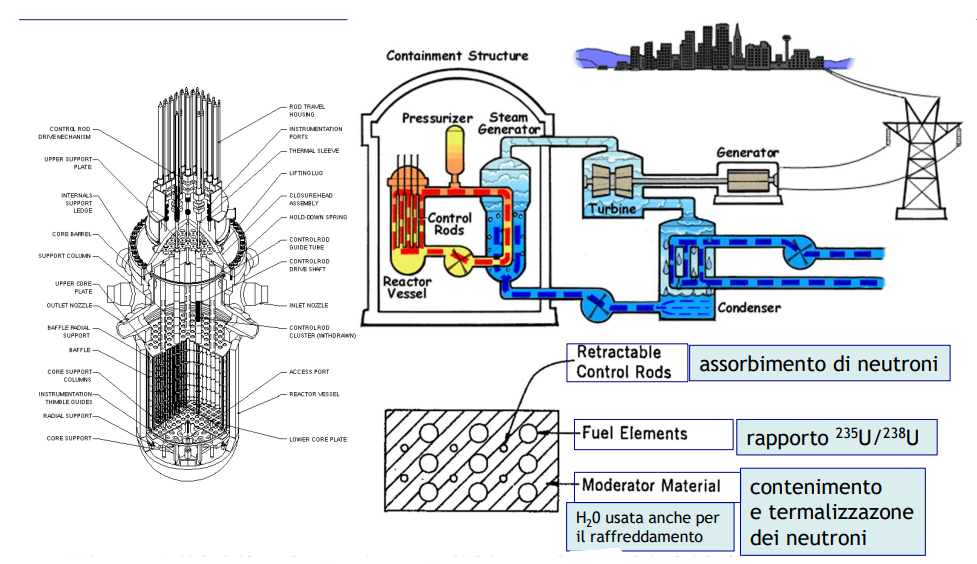
\includegraphics[scale=0.7]{Lezione5/cent.png} 
\end{figure}
Sostanzialmente un reattore ha una parte dove avviene la reazione nucleare in cui viene prodotto il calore. Questo calore viene in qualche modo trasferito in energia meccanica che viene poi convertita in energia elettrica. La zona in cui avviene la fissione è costituita da elementi di combustibile (pastiglie) di uranio in cui è importante il rapporto tra $\ch{^{235}U}/\ch{^{238}U}$. Attorno a queste pastiglie c'è un materiale che tiene separate le pastiglie di combustibile. Questo materiale viene inserito per far interagire i neutroni e diminuire la loro energia. Quello che mi serve per portare l'energia dei neutroni dall'energia di produzione all'energia termica che è quella che mi permette di raggiungere la zona in cui la sezione d'urto della fissione è maggiore. Questo \textbf{moderatore} ha anche la funzione di contenere i neutroni ed evitare che escano dalla regione di reazione. Questi due sono elementi fissi nella mia struttura. Successivamente c'è un \textbf{sistema di controllo} costituito da delle barre costituite da un materiale in grado di assorbire i neutroni che mi permette di regolare l'assorbimento di neutroni per mantenere il prodotto $\nu q$ costante. Queste barre posso aggiungerle e toglierle in base alle necessità.
\subsection{Sezione d'urto}
Consideriamo adesso una massa di uranio naturale: le frazioni dei due isotopi sono:
\begin{itemize}
    \item $\ch{^{238}U}$: $f=99.3\%$;
    \item $\ch{^{235}U}$: $f=0.7\%$.
\end{itemize}
Consideriamo un neutrone di energia cinetica $T=2\,MeV$ con $\beta=\sqrt{2T/m_n}=0.065$ (valgono ancora le approssimazioni non relativistiche). A questa energia, le sezioni d'urto totali di neutrone su $\ch{^{238}U}$ o $\ch{^{235}U}$ sono circa uguali: $\sigma_{tot}=7\,\text{barn}$. Ricordo che $1\,\text{barn}=10^{-24}\,cm^2$. Se noi prendiamo un quadrato di lato $1\,fm=10^{-15}\,m$ e quindi sono $10^{-13}\,cm$. Quindi $(1\,fm)^2=10^{-25}\,cm^2$. Quindi un barn è un qualcosa 100 volte più grande di un quadratino di lato $1\,fm$. Pensando alla dimensione di un nucleo pesante che è circa $6-7\,fm$.

In generale, se si usa una miscela di sostanze, ciascuna con frazione $f_i$, si definisce una sezione d'urto media:
\begin{equation*}
    \Bar{\sigma}=\sum f_i\sigma_i
\end{equation*}
Per l'Uranio naturale ($\rho=19.05\,g/cm^3$ e $A=238$) il numero di atomi per unità di volume è $n_T=4.8\times10^{28}\,\text{atomi}/m^3$. Otteniamo un libero cammino medio (distanza tra due collissioni):
\begin{equation*}
    \lambda=\frac{1}{\sigma n_T}=0.03\,m
\end{equation*}
Il tempo medio fra due collisioni è quindi:
\begin{equation*}
    t_c=\frac{\lambda}{v}=\frac{\lambda}{\beta c}=4.6\times10^{-9}\,s
\end{equation*}
%IMMAGINE ui uii
\begin{figure}[htp!]
  \centering
  
\includegraphics[scale=0.6]{Lezione5/ui.png}
  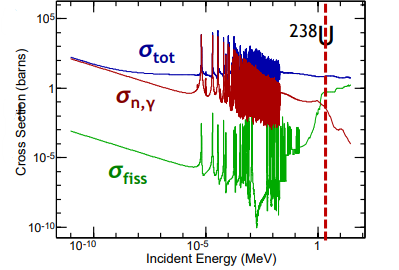
\includegraphics[scale=0.9]{Lezione5/uii.png} 
\end{figure}

Quindi ad ogni collisione il neutrone può: indurre una fissione, con probabilità:
\begin{equation*}
    p_{fiss}=\frac{\Bar{\sigma}_{fiss}}{\Bar{\sigma}_{tot}}
\end{equation*}
(da notare che le sezioni d'urto in gioco sono sempre medie in quanto abbiamo sempre a che fare con miscele di uranio-238 e uranio-235). Venir catturato con emissione di $\gamma$:
\begin{equation*}
    p_{n,\gamma}=\frac{\Bar{\sigma}_{n,\gamma}}{\Bar{\sigma}_{tot}}
\end{equation*}
e di conseguenza il neutrone non è più disponibile a far avvenire una fissione o, invece, subire una collisione elestica o anelastica con perdita di energia (facendo $1-$ la probabilità dei due eventi precedenti) e questo processo è anche quello con maggiore probabilità (sezione d'urto maggiore ottenuta dalla differenza tra la sezione d'urto totale e quella della cattura neutronica e di fissione). Nel grafico si vede una zona in cui la struttura è molto complicata con vari picchi. Quella è la struttura che indica la possibilità di eccitare livelli nucleari e quindi se ho l'energia giusta per far cambiare livelli energetici al nucleo ho picchi della sezione d'urto. In $U$ naturale, la sezione d'urto media è circa quella di $\ch{^{238}U}$. Per un neutrone di $2\,MeV$ il numero di diffusioni prima di un'interazione distruttiva $\Bar{n}=1/(p_{fiss}+ p_{n,\gamma})$ [dimostrazione nelle slide] (cioè il numero medio di collisioni prima di indurre una fissione o di venir catturato). Quindi è difficile che un neutrone colpendo un atomo avvenga subito la fissione. Ci arriverà dopo $\Bar{n}$ collisioni. La probabilità di indurre una fissione dopo i vari urti è quindi:
\begin{equation*}
    q=\frac{p_{fiss}}{p_{fiss}+p_{n,\gamma}}
\end{equation*}
Per questo motivo l'Uranio-238 non è un ottimo combustibile in quanto dopo un po' di collisioni il neutrone perde energia e, guardando il grafico, si nota che potrebbe arrivare nella zona in cui la sezione d'urto della fissione precipita e quindi la probabilità che questo accada diventa sempre più piccola (vedere grafico). Ad ogni urto l'energia del $n$ diminuisce. Quello che succede però è che se si fanno i calcoli a circa $2\,MeV$ è circa $1$. Prima di interagire faccio un sacco di collissioni elastiche e in questo modo il neutrone perde un sacco di energia. Non appena il neutrone scende sotto la soglia di energia di $2\,MeV$ (e gli bastano poche collisioni) la sua sezione d'urto per fissione diventa trascurabile e quindi diventa $q<<1$. Per cui quello che succede è che i neutroni appena emessi dalla fissione se beccassero subito un nucleo potrebbero indurre subito ad una fissione mentre in realtà il processo di fissione non è il più probabile ma è quello di fare una collisione elastica in cui il nucleo si prende un po' di energia ma il neutrone la perde. Dopo poco il neutrone perde tutta l'energia e quindi non ha più modo di innescare il processo di fissione nell'Uranio-238.

Quindi abbiamo discusso il caso in cui i neutroni (ad alta energia) che vengono prodotti dalla fissione questi neutroni vengono fuori con l'energia del $MeV$ potrebbero indurre una fissione salvo il problema che prima di indurla fanno scattering e facendo scattering con il materiale, perdono energia e scendono sotto la linea di soglia. La soluzione è aspetare che questi neutroni perdano energia con queste collisioni. Se questi raggiungono l'equilibrio termico, la situazione cambia qualitativamente:
%IMMAGINE rt tr
\begin{figure}[htp!]
  \centering
  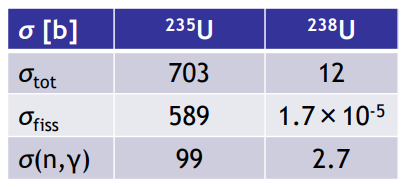
\includegraphics[scale=0.6]{Lezione5/rt.png}
  
\includegraphics[scale=0.8]{Lezione5/tr.png} 
\end{figure}
Le sezioni d'urto sono molto diverse (anche quella di scattering)
\begin{equation*}
    T=23\,meV \quad \beta=7\times10^{-6}
\end{equation*}
Visto che le sezioni d'urto di uranio-235 e uranio-238 sono molto diverse bisogna tener conto del peso che ciascun componente ha con la corrispettiva sezione d'urto. In $U$ naturale:
\begin{equation*}
    f \text{ di } \ch{^{235}U}=0.7\%
\end{equation*}
La sezione d'urto di fissione sull'uranio naturale contribuisce solamente il 235 in quanto il 238 è praticamente nullo ($10^{-5}$)
\begin{equation*}
    \Bar{\sigma}_{fiss}=0.007\times 589\,b=4.1\,b
\end{equation*}
Nella sezione d'urto di cattura elettronica invece è presente il contributo di entrambi gli isotopi.
\begin{equation*}
    \Bar{\sigma}_{n,\gamma}=0.007\times99\,b+0.993\times2.7\,b=3.4\,b
\end{equation*}
Quindi la probabilità di fissione causati da neutroni termici sull'uranio naturale è:
\begin{equation*}
    q=\frac{\Bar{\sigma}_{fiss}}{\Bar{\sigma}_{n,\gamma}+\Bar{\sigma}_{fiss}}=0.55
\end{equation*}
Sostanzialmente nell'uranio naturale circa il $55\%$ di neutroni termici possono indurre ad una fissione. Poichè $\nu\approx2.4$, $\nu q>1$ e quindi si può avere una reazione a catena. Il primo reattone nucleare è stato costruito da Fermi nel 1938 a Chicago. 

Quindi ora il problema è prendere i neutroni che vengono prodotti dalla fissione e portarli all'energia termica e per fare questo utiliziamo un moderatore. Oltre alla necessità di avere un moderatore per portare i neutroni alla energia termica c'è bisogno di avere uranio arricchito. Dobbiamo aumentare la presenza di $\ch{^{235}U}$ per aumentare $q$.
\subsection{Massa critica}
Abbiamo visto che un $n$ effettua molte collisioni prima di essere catturato o indurre fissione, la distanza tra queste collisioni è il libero cammino medio:
\begin{equation*}
    \Bar{n}=\frac{1}{p_{fiss}+p_{n,\gamma}}\qquad \lambda=\frac{1}{\sigma_{tot}n_T}
\end{equation*}
Essendo questo un processo casuale, \textbf{random walk}, la distanza media percorsa dal $n$ rispetto al punto di produzione è:
\begin{equation*}
    	\left \langle l \right \rangle =\lambda\sqrt{\Bar{n}}
\end{equation*}
Se il blocco di combustibile ha una dimensione minore di tale distanza, alcuni $n$ usciranno senza aver fatto in tempo ad interagire. Esiste quindi una dimensione minima $L_{min}$ che il reattore deve avere perchè la reazioni possa autosostenersi. Di conseguenza un valore minimo di volume $V_{min}\sim L_{min}^3$, e di massa $\rho V_{min}$ e quindi una \textbf{massa critica}. Il valore esatto dipende da geometria, combustibile e molti altri fattori. Quindi in questo quando si parla di massa critica non è tanto un concetto legato al peso ma legato al cammino libero medio!
\subsection{Rallentamento dei neutroni}
I neutroni rallentano (perdono energia) in seguito alle collisioni con i nuclei del materiale in cui si muovono. Quando il neutrone è veloce una causa di rallentamento è una interazione inelastica:
\begin{equation*}
    n+A\,\to\, A^*+n
\end{equation*}
Nel bilancio energetico della reazione entra anche l'energia del \textbf{livello eccitato} che pertanto non è più disponibile come enrgia cinetica del neutrone finale. Ora si nota che tornano tutti i conti nell'interazione a due corpi. Quando io ho un neutrone che va su un bersaglio che è decine o centinaia di volte più grande l'energia cinetica che viene passata al bersaglio è piccola, questo perchè $T_A$ è molto piccolo quindi l'energia del neutrone iniziale è uguale
\begin{equation*}
    T_n=T_A+E^*_A+T_n' \qquad T_n'\approx T_n-E^*_n
\end{equation*}
Questo succede nella regione in cui sono presenti i vari picchi.

Questo meccanismo diventa rapidamente inefficace quando l'energia dei neutroni diventa insufficiente per eccitare il bersaglio. Infatti, come dal grafico, sotto il decimo di $MeV$ non ho più una struttura con picchi (sezione d'urto molto alte dovute all'eccitazione) ma abbiamo un andamento continuo dovuto al fatto che si è bloccata la perdita di energia per eccitazione ma c'è solo la collisione di tipo elastico. Quindi il grosso del passaggio da $1\,MeV$ (quando vengono prodotti i neutroni) all'energia termica (attorno a $10^{-7}\,MeV$) diventa importante e il meccanismo più efficace lo \textbf{scattering elastico}[vedi slide].
Dopo vari calcoli si arriva alla relazione:
\begin{equation*}
    \frac{dN}{dE_3}=\frac{dN}{d\cos{\theta^*}}\frac{d\cos{\theta^*}}{dE_3} \qquad\frac{d\cos{\theta^*}}{dE_3}=\frac{(A+1)^2}{2A}\frac{1}{E_1} \qquad \frac{dN}{d\cos{\theta^*}}=\text{cost}=\frac{1}{2}
\end{equation*}
Introducendo $x=E_3/E_1$ si ottiene:
\begin{equation*}
    \frac{dN}{dx}=\frac{(A+1)^2}{4A}
\end{equation*}
Vediamo quindi che dopo l'urto la distribuzione dell'energia del neutrone è uniforme:
%IMMAGINE yu
\begin{figure}[htp!]
  \centering
  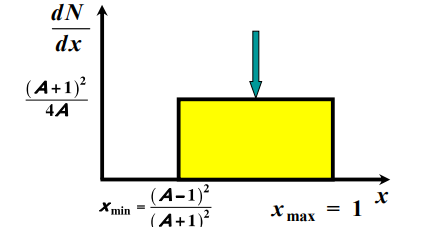
\includegraphics[scale=0.7]{Lezione5/yu.png} 
\end{figure}
è immediato calcolare il valor medio:
\begin{equation*}
    \left \langle x \right \rangle =\left \langle \frac{E_3}{E_1} \right \rangle =\frac{1}{2}(x_{min}+x_{max})=\frac{A^2+1}{(A+1)^2}
\end{equation*}
La formula trovata ci permette di capire quali materiali funzionano meglio per rallentare i neutroni, dopo l'urto l'energia del neutrone è uniformemente distribuita fra:
\begin{equation*}
    \frac{E_{3min}}{E_1}=\frac{(A-1)^2}{(A+1)^2} \qquad \frac{E_{3max}}{E_1}=1
\end{equation*}
Se il nucleo è leggero l'intervallo è largo, ad esempio con l'idrogeno $A=1$, si ha che $0\le x\le1$ e quindi in questo caso in un singolo urto il neutrone può perdere molta energia. Se il nucleo è pesante l'intervallo è molto più stretto, ad esempio l'uranio $A=238$, si ha $0.98\le x\le1$ e quindi sostanzialmente la mia variazione di energia è molto limitata e quindi mi servono a tanti urti per portare i neutroni ad energia termica. Da qui si capisce \textbf{per rallentare i neutroni occorre utilizzare nuclei leggeri}. 

Ci poniamo adesso la domanda: quante collisioni sono necessarie per raggiungere una energia termica? Supponiamo che il neutrone faccia una succesione di urti,  nel passo $k-1\to k$ l'energia varia da $E_{k-1}$ a $E_k$. Il rapporto $x=E_k/E_{k-1}$ è distribuito uniformemente. I limiti della distribuzione dipendono dal nucleo ($A$)
\begin{equation*}
    \frac{E_n}{E_0}=\frac{E_n}{E_{n-1}}\frac{E_{n-1}}{E_{n-2}}\ldots\frac{E_2}{E_1}\frac{E_1}{E_0}=	\prod_{k=1}^n \frac{E_k}{E_{k-1}}
\end{equation*}
Conviene considerare il logaritmo di questa espressione:
\begin{equation*}
    \ln\left(\frac{E_n}{E_0}\right)=\sum_{i=0}^n\ln\left(\frac{E_i}{E_{i-1}}\right)
\end{equation*}
Ancora una volta notiamo che $x=E_k/E_{k-1}$ ha sempre la stessa distribuzione. Dal momento che abbiamo molti urti e che la distribuzione è sempre la stessa possiamo utilizzare il teorema del limite centrale.
\begin{equation*}
    \left \langle \sum_{i=0}^n\ln\left(\frac{E_i}{E_{i-1}}\right) \right \rangle=n\left \langle \ln\left(\frac{E_f}{E_i}\right) \right \rangle
\end{equation*}
Dove $E_i$ è l'energia prima dell'urto e $E_f$ l'energia dopo l'urto. Utilizzando questo risultato:
\begin{equation*}
    \left \langle \ln\left(\frac{E_n}{E_0}\right) \right \rangle =n\left \langle \ln\left(\frac{E_f}{E_i}\right)\right \rangle 
\end{equation*}
Possiamo stimare il numero di collisioni necessarie. Mi manca solo il valor medio di questo logaritmo.
\begin{equation*}
    \left \langle \ln\left(\frac{E_f}{E_i}\right)\right \rangle=\frac{(A_1)^2}{2A}\ln{\left(\frac{A+1}{A-1}\right)}-1 \qquad n=\frac{\left \langle \ln\left(\frac{E_n}{E_0}\right) \right \rangle}{\left \langle \ln\left(\frac{E_f}{E_i}\right)\right \rangle}
\end{equation*}
\subsection{Moderatori}
Utilizzando ora queste formule possiamo trovare e confrontare i vari materiali per il loro uso come \textbf{moderatori}. Ad esempio per "raffreddare" da $2\,MeV$ a $0.02\,eV$ un neutrone:
\begin{itemize}
    \item Idrogeno $H$: $A=1$  $n=18$
    \item Deuterio $\ch{^2H}$: $A=2$ $n=25$
    \item Grafite $\ch{^{12}C}$: $A=12$ $n=115$
\end{itemize}
Ora qualcuno potrebbe dire "ah bellissimo allora il miglior moderatore è l'idrogeno perchè mi bastano pochissime collissioni per portare i neutroni all'energia termica" in realtà non è l'unica cosa che devo considerare ma devo tener conto che nelle collisioni con il moderatore (in cui il processo dominante è la diffusione elastica) però ho anche la cattura neutronica! I materiali devono anche essere cconfrontati sulla base delle loro sezioni d'urto elastiche e di assorbimento.
%IMMAGINE fg
\begin{figure}[htp!]
  \centering
  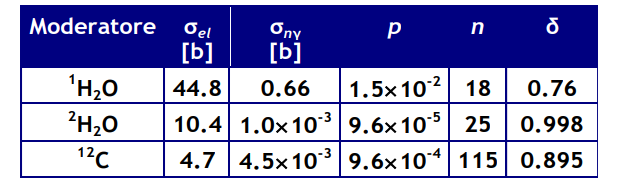
\includegraphics[scale=0.7]{Lezione5/fg.png} 
\end{figure}
Anche se la probabilità di cattura neutronica è piccola bisogna tener conto che avvengono molte collisioni. Dalla tabella si nota che sebbene mi servono solo $18$ collissioni per arrivare all'energia termica ho il $78\%$ di probabilità che il neutrone venga assorbito e quindi perdo il $24\%$ di neutroni. Se prendo l'acqua pesante quello che succede è che la sezione d'urto di cattura neutronica è molto più bassa e quindi sopravvivono molti più neutroni (anche se il numero di collisioni è maggiore). Infatti i primi reattori nucleari usavano acqua pesante proprio per questo motivo. [Vedere le slide per approfondimento del controllo della catena].
\subsection{Sicurezza del reattore}
Una caratteristica molto importante dei reattori è la variazione del paramentro $k=\nu q$ con la quantità del materiale refrigeratore, cosa succede se avviene una perdita nel moderatore/refrigeratore? Il risultato è la combinazione di due effetti: se la quantità di moderatore \textbf{diminuisce} l'energia dei neutroni è più alta, i neutroni quindi rilasciano un'energia maggiore e la temperatura aumenta. D'altro canto se l'enegia dei neutroni è più alta la probabilità di fissione diminuisce, quindi la potenza del reattore diminuisce e quindi la temperatura diminuisce. Il reattore infatti è sicuro se il secondo effetto prevale sul primo:
\begin{equation*}
    \frac{dk}{dT}<0
\end{equation*}
\subsection{Sommario}
In un evento di fissione si libera $\sim1\,MeV/\text{nucleone}$. \textbf{Energia di legame} $\sim7\, MeV/\text{nucleone}$ per $A\sim200$ ($\sim8\,MeV/\text{nucleone}$ in media per $A>60$). La fissione spontanea è energeticamente possibile ma molto rara: dalle \textbf{probabilità di decadimento}, potenza prodotta $10^{-13}\,W$ questo perchè necessitiamo di superare una \textbf{barriera di potenziale}. La fissione può venir indotta dalla cattura neutronica (ci da un sacco di energia in più che ci permette di superare la barriera di potenziale che arriva dall'energia di legame del neutrone catturato). I materiali fissili hanno $A$ dispari e sfruttano il termine $a_5$ della \textbf{relazione di Bethe-Weizs\"acker} che aumenta tale energia. Infatti se ho un materiale con $A$ dispari (con $Z$ pari e $N$ dispari) così quando catturo il neutrone ha quel guadagno sull'energia di legame che mi da la possibilità di avere dell'energia liberata in più per superare la barriera di potenziale. Il mantenimento della fissione si basa sul controllo di $n$: equilibrio tra la \textbf{sezione d'urto} per fissione e cattura ($n,\gamma$) infatti se ho troppa fissione la mia reazione tende ad essere troppo veloce mentre se ho troppa cattura neutronica la mia reazione tende a spegnersi quindi si gioca tutto con il corretto bilanciamento dei due processi. 